\begin{blocksection}
\question Define the function \lstinline$factor_tree$ which returns a \emph{factor tree}. Recall that in a factor tree, multiplying the leaves together is the prime factorization of the root, $n$. \\

 \begin{center}
 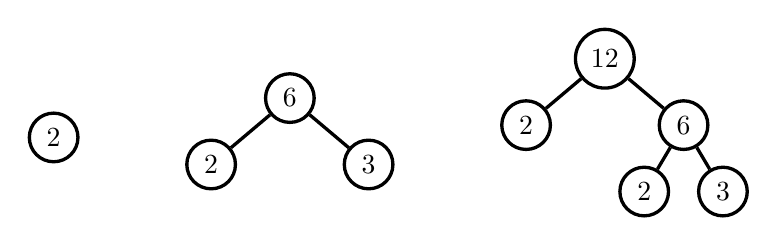
\begin{tikzpicture}[very thick,level/.style={sibling distance=20mm/#1},level distance=24pt]
 \node[circle, draw] at (0,-1){$2$};
 \node[circle, draw] at (3,-0.5){$6$}
 child {
     node[circle, draw]{$2$}
 }
 child {
     node[circle, draw]{$3$}
 };
 \node[circle, draw]at (7,0){$12$}
 child {
     node[circle, draw]{$2$}
 }
 child {
     node[circle, draw]{$6$}
     child {
         node[circle, draw]{$2$}
     }
     child {
         node[circle, draw]{$3$}
     }
 };
 \end{tikzpicture}
 \end{center}




\begin{lstlisting}
def factor_tree(n):

    for i in ______________________:

        if ________________________:

            return tree(_____, _____________________________)

    _______________________________
\end{lstlisting}

\begin{solution}[0.5in]
\begin{lstlisting}
    for i in range(2, n):
        if n % i == 0:
            return tree(n, [factor_tree(i), factor_tree(n // i)])
    return tree(n)
\end{lstlisting}
\end{solution}
\end{blocksection}
